\documentclass{article}
\usepackage[UTF8]{ctex}
\usepackage{pythonhighlight}

% Language setting
% Replace `english' with e.g. `spanish' to change the document language
\usepackage[english]{babel}
\usepackage{float}
% Set page size and margins
% Replace `letterpaper' with `a4paper' for UK/EU standard size
\usepackage[letterpaper,top=2cm,bottom=2cm,left=3cm,right=3cm,marginparwidth=1.75cm]{geometry}

% Useful packages
\usepackage{amsmath}
\usepackage{graphicx}
\usepackage[colorlinks=true, allcolors=blue]{hyperref}

\title{数逻实验报告Lab4}
\author{雷远航}
 
\begin{document}

\maketitle

\begin{abstract}
实验项目:EDA实验平台与实验环境运用
\end{abstract}

\section{操作方法与实验步骤}

\subsection{用verilog语言描述电路逻辑功能}

\subsubsection{在ISE中创建工程}

首先在ISE中完成对工程的创建,并向其中导入Verilog代码


\subsubsection{对代码进行仿真运行}

导入仿真激励代码,进行仿真运行,得到波形图
\begin{figure}[H]
	\centering
	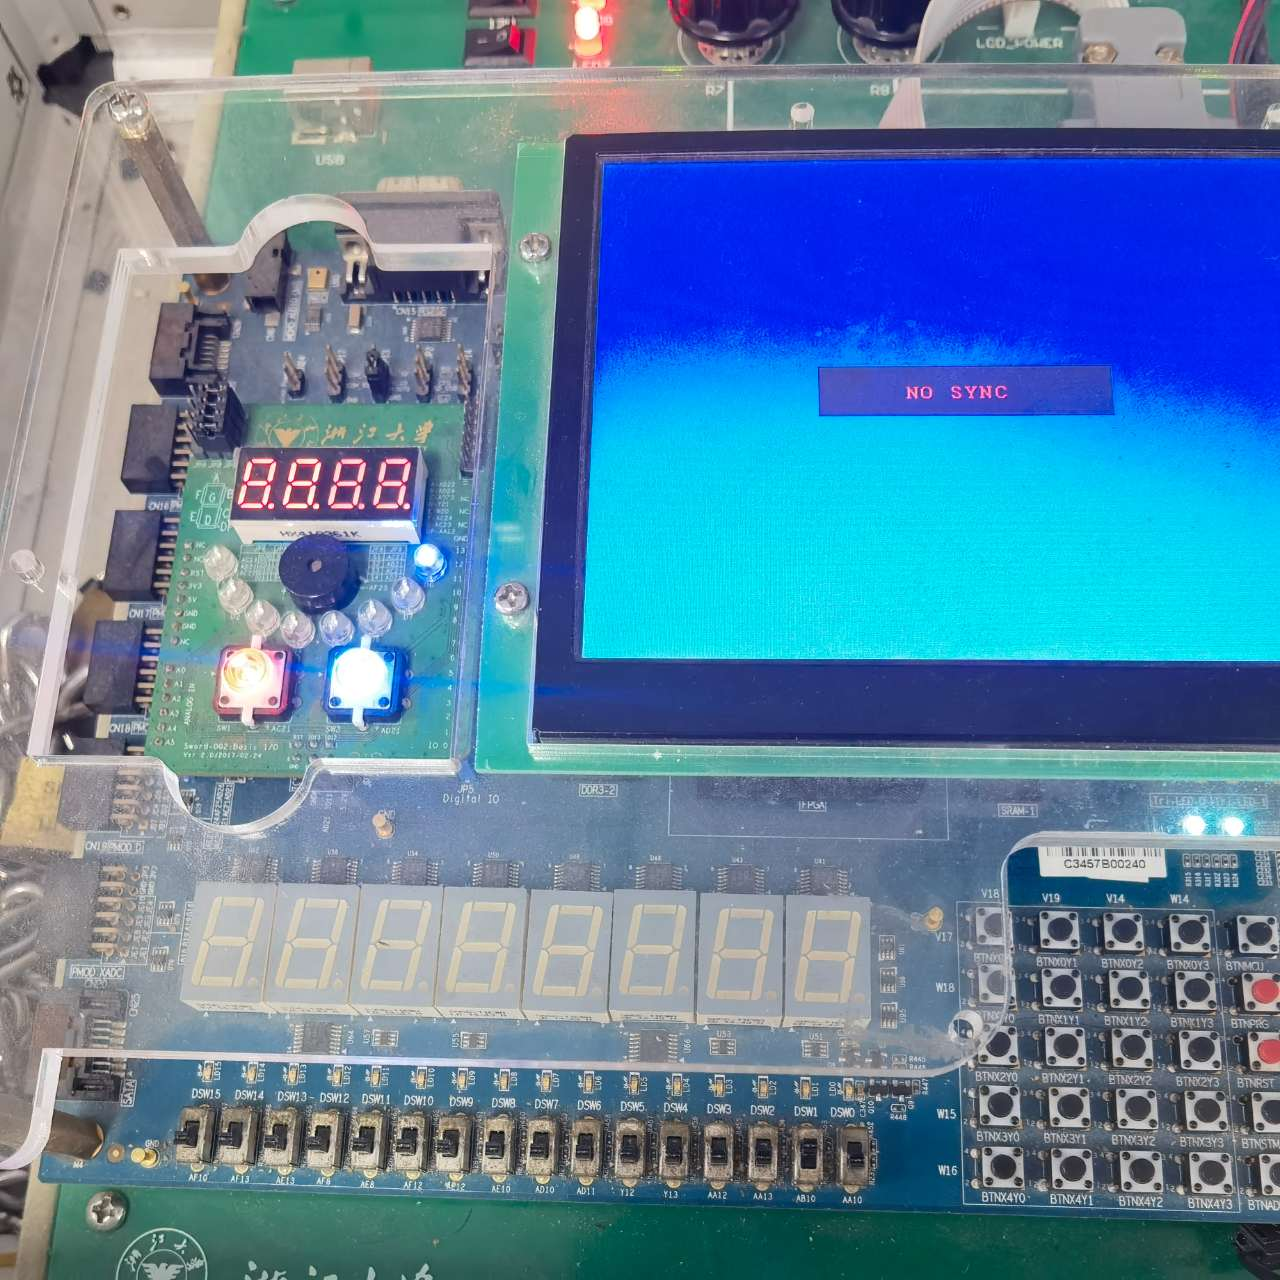
\includegraphics[width=0.5\textwidth]{1.jpg}
	\caption{\label{Lab4}创建工程}
	\end{figure}

\subsubsection{完成全部实验操作}

完成Synthesize,Implement Design,Generate Programming File,将生成的bit文件下载到sword实验板上





\subsection{以图形方式输入逻辑功能描述}

\subsubsection{创建工程并绘图}


\subsubsection{进行仿真运行}

导入仿真激励代码,进行仿真运行,得到波形图


\subsubsection{完成全部实验操作}

完成Synthesize,Implement Design,Generate Programming File,将生成的bit文件下载到sword实验板上

\section{实验结果描述与分析}

\subsection{verilog实验结果}

当拨动其中一个开关时,信号灯闪亮,在不进行其他操作时,在一段时间内灯自动熄灭


在打开一个开关,信号灯闪亮时再次拨动另一个开关,信号灯关闭,并且此过程又一定的延时现象


\subsection{图形化实验结果}

当打开一个开关时,信号灯闪亮;打开两个开关时信号灯熄灭,并且此过程并没有延时现象出现





\section{讨论与心得}

通过本次实验我熟悉了ISE平台的使用流程和方法,通过对verilog教程的学习大致了解了verilog语言的编写方法,实验主要遇到的障碍是:1.在没有明确实验报告的要求之前参照优秀报告,进行了很多不必要的截图,耽误了比较多的时间. 2.在画图时画了总线,并且没用正确画出,导致开始的时候check一直错误,把总线删除后解决了问题

\section{Bonous}

\subsection{Verilog工程理解}
LampCtrl是实现全部功能的基本模块,通过parameter CMAX,和reg cout的配合使用可以实现时序电路的功能,控制在闪亮一段时间后自动熄灭,总的输出由F进行,根据输入响应所得到的结果是w,通过时序判断才是最终的结果F

testbench的作用是对自己所写的module进行结果的测试,进行正确性的验证,testbench通过对模块的实例化,不断改变输入的值,最终通过生成的波形图进行结果的验证

\subsection{控制LED暂缓熄灭的时间}
对parameter CMAX进行修改,若要将熄灭时间变为原来的2倍、4倍、1/2倍、1/4倍,就将CMAX变为原来的2倍、4倍、1/2倍、1/4倍,同时也要对代表位数的CNUM做相应的调整

\subsection{对实验给出的testbench得到的波形进行说明}
对于verilog实现的波形图首先测试时等待了一定的时间,然后将S1设置为1,这样输出F就是1,在持续一段时间后由于CMAX的控制在接下来的等待时间下最终F会变回1

图像实现的测试由于没有实现时序电路的功能因此当输入发生变化时输出会立即进行响应变化

\subsection{对slides: First Look at Verilog建议}
可以在教程中多添加一些链接到HDLBits的相应练习题的网址,这样可以边学习边练习效果会更好



\end{document}
